\documentclass{article}
\usepackage{tikz}

\begin{document}

\begin{figure}[h]
    \centering
    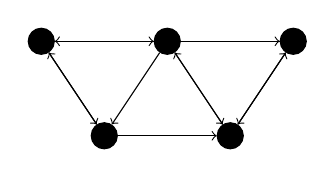
\begin{tikzpicture}[scale=0.8]
        % Define nodes
        \node (A) at (0,0) [circle,draw,fill=black] {};
        \node (B) at (2,0) [circle,draw,fill=black] {};
        \node (C) at (4,0) [circle,draw,fill=black] {};
        \node (D) at (1,-1.5) [circle,draw,fill=black] {};
        \node (E) at (3,-1.5) [circle,draw,fill=black] {};

        % Draw edges
        \draw[->] (A) -- (B);
        \draw[->] (B) -- (C);
        \draw[->] (C) -- (A);
        \draw[->] (A) -- (D);
        \draw[->] (B) -- (E);
        \draw[->] (D) -- (E);
        \draw[->] (E) -- (C);

        % Additional edges to maintain symmetry
        \draw[->] (B) -- (D);
        \draw[->] (C) -- (E);
        \draw[->] (D) -- (A);
        \draw[->] (E) -- (B);
    \end{tikzpicture}
    \caption{Non-Bipartite Oriented Graph with 3-Symmetric Spectrum}
    \label{fig:nonbipartitegraph}
\end{figure}

\end{document}